\subsection{Constructionism}

Programming is an activity that deals primarily with the construction
of abstract structures from ideas. This process and some of its encompassing
theories are usually neglected or just fade into the conceptual
background. This void is filled by constructionism, a learning theory
developed by Seymour Papert and his colleagues that:

\begin{quote}
  ... shares constructivism's connotation of learning as ``building
  knowledge structures'' irrespective of the circumstances of the
  learning. It then adds the idea that this happens especially
  felicitously in a context where the learner is consciously engaged in
  constructing a public entity, whether it's a sand castle on the beach
  or a theory of the universe.
  \cite{education:papert__situating_constructionism}
\end{quote}

The proponents of this theory were the front-runners of using
computers as a \emph{personal media}. They did that in order to
propose an alternative to instructionism and technocentrism. Those
ideas can be summarized in the claim that \emph{``To get better
  education, we must improve instruction. And if we're going to use
  computers, we'll make the computers do the
  instructon.''}. \cite{education:papert__constructionism_instructionism} 

Constructionism's alternative consists of using media, technology, and
social environments as scaffolds to the conceptual structures that is
to be built by people in the active role of their education. This
education consisted initially of children learning math supported by
constructionism's answer to traditional math curricula, Logo. 

\begin{wrapfigure}{r}{40mm}
  \begin{center}
    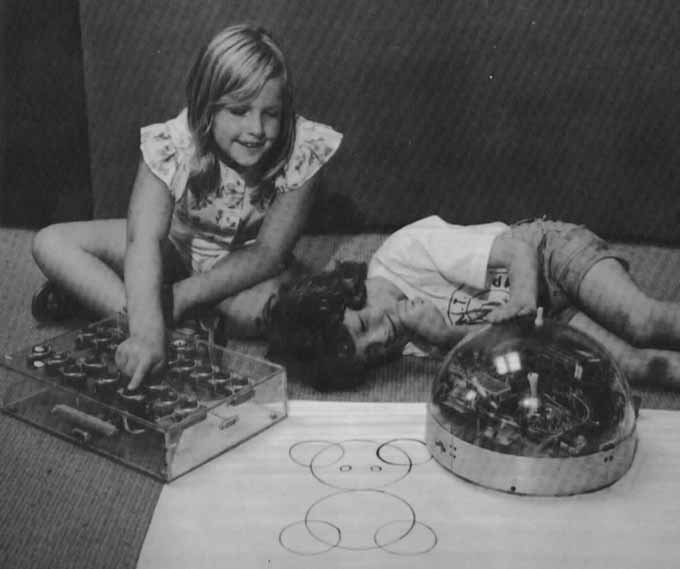
\includegraphics[scale=0.7]{images/mindstorms_turtle.jpg}
  \end{center}
  \caption{Children programming in logo. \cite{education:papert_mindstorms}}
\end{wrapfigure}

Logo profoundly influenced modern computer languages and environments
through the heavy impact it had on the development of the Smalltalk
system:

\begin{quotation}
  
  I finally visited Seymour Papert, Wally Feurzig, Cynthia Solomon and
  some of the other original researchers who had built LOGO and were
  using it with children in the Lexington schools. Here were children
  doing real programming with a specially designed language and
  environment. As with Simula's leading to OOP, this encounter finally
  hit me with what the destiny of personal computing really was going
  to be. Not a personal dynamic vehicle, as in Engelbart's metaphor
  opposed to the IBM ``railroads'', but something much more profound: a
  personal dynamic medium. With a vehicle one could wait until high
  school and give ``drivers ed'', but if it was a medium, it had to
  extend into the world of childhood. 
  \cite{smalltalk:kay_alan__early_history_smalltalk}

\end{quotation}
